Vengono riportati in questa sezione dei diagrammi di sequenza, al fine di illustrare meglio l'architettura del server.\\
Il diagramma riportato in figura~\ref{fig:seq1} mostra il flusso delle operazioni causate da un'azione dell'utente che non va a modificare i dati nel database. Si vede che l'ordine delle chiamate parte dal livello di presentazione e viene inoltrato nei livelli inferiori fino a quando viene effettivamente chiamato il metodo richiesto. Nei ritorni ci sono dei controlli che sono stati inseriti per verificare l'esito (successo/fallimento) dell'operazione in maniera che esso potesse essere segnalato. Le regole per la comunicazione tra i livelli sono uniformi e standardizzate. \\
\begin{figure}[!h]
\centering
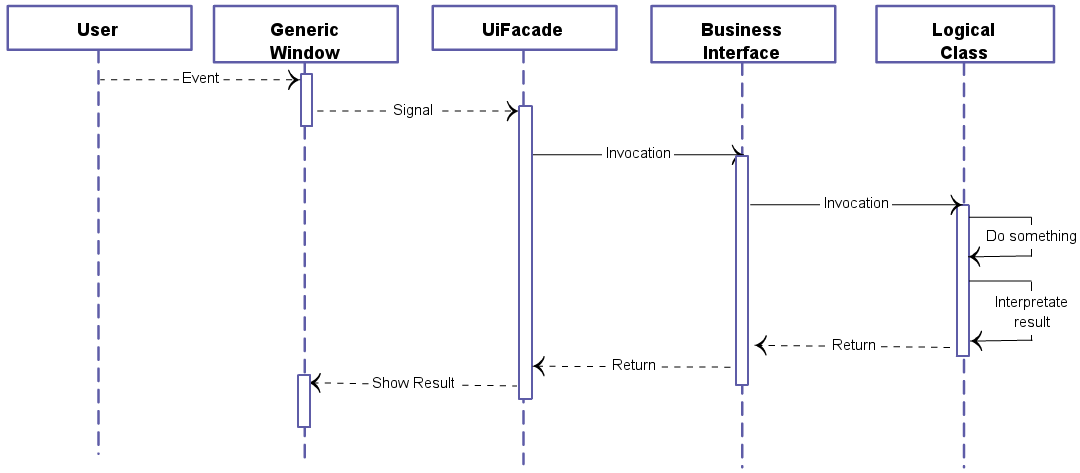
\includegraphics[scale=0.4]{./images/seq1.png}
\caption{Diagramma di sequenza, generica richiesta dell'utente}
\label{fig:seq1}
\end{figure}
Similmente il diagramma in figura~\ref{fig:seq2} riporta il flusso delle operazioni quando è coinvolto il livello dell'accesso ai dati.
\begin{figure}[!h]
\centering
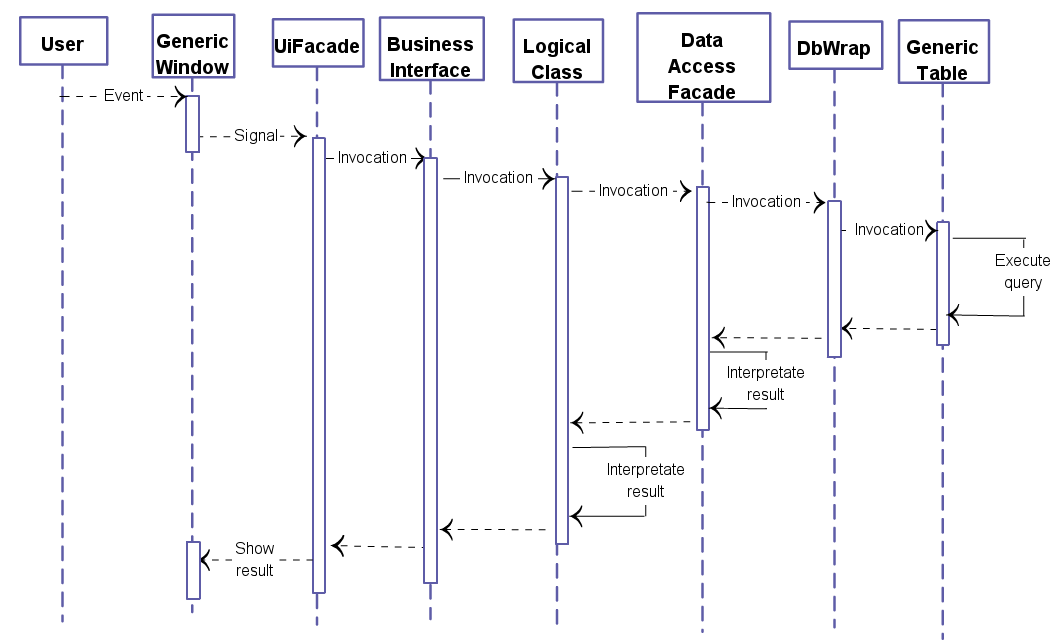
\includegraphics[scale=0.4]{./images/seq2.png}
\caption{Diagramma di sequenza, generica richiesta utentei di  modifica ai dati}
\label{fig:seq2}
\end{figure}